% Created 2021-01-10 Sun 16:54
% Intended LaTeX compiler: pdflatex
\documentclass[11pt]{article}
\usepackage[utf8]{inputenc}
\usepackage[T1]{fontenc}
\usepackage{graphicx}
\usepackage{grffile}
\usepackage{longtable}
\usepackage{wrapfig}
\usepackage{rotating}
\usepackage[normalem]{ulem}
\usepackage{amsmath}
\usepackage{textcomp}
\usepackage{amssymb}
\usepackage{capt-of}
\usepackage{hyperref}
\author{sergisi}
\date{\today}
\title{Dec16}
\hypersetup{
 pdfauthor={sergisi},
 pdftitle={Dec16},
 pdfkeywords={},
 pdfsubject={},
 pdfcreator={Emacs 27.1 (Org mode 9.5)}, 
 pdflang={English}}
\begin{document}

\maketitle
\tableofcontents

\begin{center}
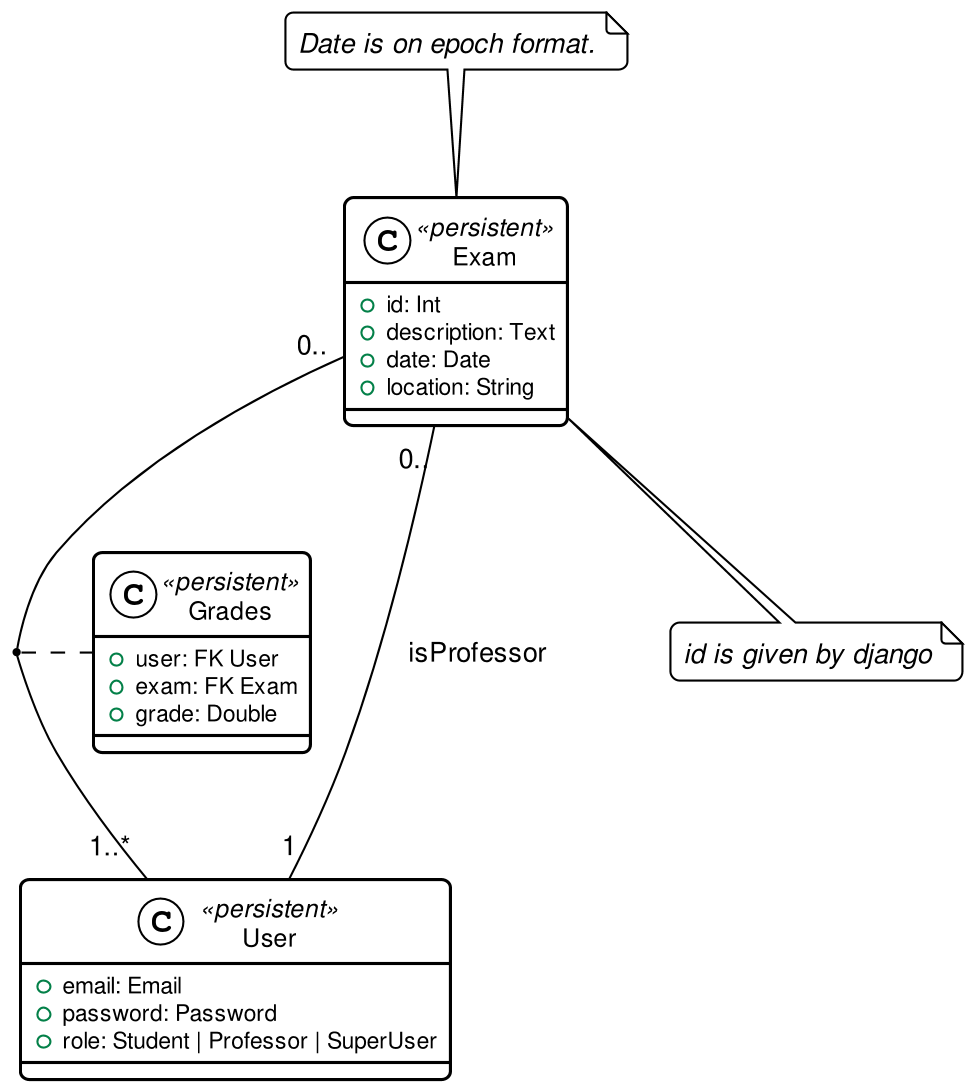
\includegraphics[width=.9\linewidth]{img/message_passing.png}
\end{center}

\section{Coses a preguntar}
\label{sec:org8ea9842}
\begin{itemize}
\item Sobre time i location (Exam)
\item Datasource serveix per extraure el driver de connexió del servidor, i
aixi poder canviar de base de dades. En el nostre cas ja ho fa SQLAlchemy
(ORM), que extrau aquest tipus de connexio de SQLs. L'abstracció de quina
BD utilitzar ho farem desde l'\texttt{.env}.
\item Session es necessari? RMI qualsevol estudiant es pot connectar. Llavors,
el Professor ha de dir els alumnes que es poden connectar? O mentre sigui
un alumne es pot connectar al examen?
\end{itemize}

\section{Notes de desenvolupament}
\label{sec:org85187fa}
\begin{itemize}
\item Canviar delete dels tests d'exam, només s'ha de poder esborrar
si no té grades.
\end{itemize}

\section{Arquitectura}
\label{sec:org976cde0}
\subsection{Bàsics}
\label{sec:orgfbed975}
\begin{itemize}
\item Donar un identificador a l'exam
\item Guardar la descripció, la date/time i location
---
\item Poder borrar l'examen si no te cap nota
\item Modificar la descripció de l'examen
\item S'ha de poder buscar el contingut de l'examen amb l'id
o la descripció parcial o sencera de l'examen.
\item s'ha de poder descargar la informació de l'examen per
identificador o per llistant tots els examens
\end{itemize}

\subsection{Advanced}
\label{sec:org8807a16}
\begin{itemize}
\item S'ha de poder posar notes a un examen.
\item S'ha de poder descarregar les notes d'un estudiant.
\item S'ha de poder guardar i extreure tota la informació dels
examens / teus examens.
\item -- de la merda que utilitza
\item S'ha de poder gestionar l' accés de l'estudiant per id. (?)
\end{itemize}

\subsection{Integració}
\label{sec:org63aa53c}
\begin{itemize}
\item RMI ha de crear l'examen al ws.
\item Els estudiants han de validar l'id abans de començar
l'examen. Els hi donarà detalls de la connexió amb el
servidor.
\item S'ha de poder guardar les notes desde el WS.
\end{itemize}

\texttt{exam=exam\_id}
\begin{table}[htbp]
\label{Methods table. Preceeded by api at ngix level}
\centering
\begin{tabular}{lll}
\hline
Method & URL & What\\
\hline
get & exam/ & List d'exams\\
get & exam/\{exam\}/ & Detall de Exam (tot)\\
get & exam/search?description=\{text\}/ & Buscar descripció parcial.\\
post & exam/ & Crea exam. pk no s'ha de donar.\\
put & exam/\{exam\}/ & Modificar camps d'Exam (tots)\\
patch & exam/\{exam\}/ & Partial update.\\
delete & exam/\{exam\}/ & Deletes if professor and no grades\\
\hline
post & grades/ & Penjar nota d'un examen.\\
get & grades/\{user\}/user/ & List totes les notes d'un estudiant.\\
get & grades/ & List all grades.\\
get & grades/\{grade\textsubscript{id}\} & Detail a grade.\\
put & grades/\{grade\textsubscript{id}\} & Updates a grade.\\
patch & grades/\{grade\textsubscript{id}\} & Partially updates a grade.\\
delete & grades/\{grade\textsubscript{id}\} & Deletes a grade.\\
\hline
post & auth/login/ & Logins\\
get & auth/logout/ & Logouts\\
post & auth/logout/ & Logout\\
post & auth/password/change/ & Password change.\\
post & auth/password/reset/ & Password reset by email confirmation. Needs Email configuration\\
post & auth/password/reset/confirm/ & Password Confirmation\\
post & auth/registration/ & Register a new user.\\
post & auth/registration/verify-email & Verifies email. Needs Email configuration\\
get & auth/user/ & Reads User. Needs authentication\\
put & auth/user/ & Updates User\\
patch & auth/user/ & Partial update.\\
\hline
\end{tabular}
\end{table}
\end{document}
